\documentclass[compress]{beamer}
\usepackage{ifthen,verbatim}

\newcommand{\isnote}{}
\xdefinecolor{lightyellow}{rgb}{1.,1.,0.25}
\xdefinecolor{darkblue}{rgb}{0.1,0.1,0.7}

%% Uncomment this to get annotations
%% \def\notes{\addtocounter{page}{-1}
%%            \renewcommand{\isnote}{*}
%% 	   \beamertemplateshadingbackground{lightyellow}{white}
%%            \begin{frame}
%%            \frametitle{Notes for the previous page (page \insertpagenumber)}
%%            \itemize}
%% \def\endnotes{\enditemize
%% 	      \end{frame}
%%               \beamertemplateshadingbackground{white}{white}
%%               \renewcommand{\isnote}{}}

%% Uncomment this to not get annotations
\def\notes{\comment}
\def\endnotes{\endcomment}

\setbeamertemplate{navigation symbols}{}
\setbeamertemplate{headline}{\mbox{ } \hfill
\begin{minipage}{5.5 cm}
\vspace{-0.75 cm} \small
\end{minipage} \hfill
\begin{minipage}{4.5 cm}
\vspace{-0.75 cm} \small
\begin{flushright}
\ifthenelse{\equal{\insertpagenumber}{1}}{}{Jim Pivarski \hspace{0.2 cm} \insertpagenumber\isnote/\pageref{numpages}}
\end{flushright}
\end{minipage}\mbox{\hspace{0.2 cm}}\includegraphics[height=1 cm]{../cmslogo} \hspace{0.1 cm} \includegraphics[height=1 cm]{../tamulogo} \hspace{0.01 cm} \vspace{-1.05 cm}}

\begin{document}
\begin{frame}
\vfill
\begin{center}
\textcolor{darkblue}{\Large Status of Beam-Halo Alignment with First Beams}

\vfill
\begin{columns}
\column{0.3\linewidth}
\begin{center}
\large
\textcolor{darkblue}{Jim Pivarski}

\vspace{0.2 cm}
Alexei Safonov
\end{center}

\column{0.3\linewidth}
\begin{center}
\large
K\'aroly Banicz
\end{center}
\end{columns}

\begin{columns}
\column{0.3\linewidth}
\begin{center}
\scriptsize
{\it Texas A\&M University}
\end{center}
\column{0.3\linewidth}
\begin{center}
\scriptsize
{\it US-CMS}
\end{center}
\end{columns}

\vfill
18 September, 2008

\end{center}
\end{frame}

%% \begin{notes}
%% \item This is the annotated version of my talk.
%% \item If you want the version that I am presenting, download the one
%% labeled ``slides'' on Indico (or just ignore these yellow pages).
%% \item The annotated version is provided for extra detail and a written
%% record of comments that I intend to make orally.
%% \item Yellow notes refer to the content on the {\it previous} page.
%% \item All other slides are identical for the two versions.
%% \end{notes}

\begin{frame}
\frametitle{In a nutshell}
\small
\begin{itemize}\setlength{\itemsep}{0.15 cm}
\item Idea: tracks passing through overlap of neighboring CSC chambers yield relative position of pairs; use these to reconstruct whole ring
\item History: long succession of trial-and-error; a subtle problem!
\item Consistency check: ring must ``close,'' residuals must be centered for all pairs of chambers simultaneously
\item Methods (now that the dust has settled):
\begin{itemize}
\item Step-by-step: fix one chamber, align its neighbors, align its neighbors' neighbors\ldots\ check quality with closure
\item Matrix-based: minimize a global $\chi^2$ by solving 18 (or 36) simultaneous equations, check quality with final $\chi^2$
\end{itemize}
\item Advantages/disadvantages: step-by-step can be used when a chamber is
  missing, matrix-based more evenly distributes error \\ (and therefore typical
  errors are smaller)
\item Status: works in MC, reveals the expected 2.5~mm radial shift in cosmics data (ME+2/2, 3/2), close to working in beam-halo data
\end{itemize}
\end{frame}

%% \section*{First section}
%% \begin{frame}
%% \begin{center}
%% \Huge \textcolor{blue}{First section}
%% \end{center}
%% \end{frame}

\begin{frame}
\frametitle{Alignment details}
\small
\begin{itemize}
\item Alignment is in global $r\phi$, rather than local $x$ \\ (chambers glued to circle around the beamline, not a polygon)
\item Residuals measured perpendicular to strips (always tangent to circle)
\item Necessitates a new alignment package, a software issue to be dealt with later
\end{itemize}

\vspace{0.4 cm}
\hspace{-0.83 cm} \textcolor{darkblue}{\Large Properties of closure in this framework}

\vspace{0.2 cm}
\begin{itemize}
\item Independent of the alignment state: moving a chamber in $r\phi$
  increases residuals on one side and reduces them on the other
\item Independent of whether we align chamber $N$ to $N+1$ or align chamber $N$ to $N-1$
\item Closure is a property of fitting procedure, misalignments other
  than $r\phi$, and possibly deeper detector issues
\end{itemize}
\end{frame}

\begin{frame}
\frametitle{Results, expressed as radial shift}
\small

Lack of closure can be interpreted as increase/decrease in radius

\begin{itemize}
\item MC: all rings less than 1~mm, most $\sim$300~$\mu$m (new accomplishment)
\item Cosmics data: ME+2/1 wants to shrink 1.8~mm, ME+2/2 and 3/2 want to increase 3.5 and 3.0~mm
\begin{itemize}
\item Good (2/2 and 3/2)! There was an actual radial misalignment of 2.5~mm in ME2/2 and 3/2 (with the right sign)
\end{itemize}
\item Beam-halo data: ME+2/1 wants to shrink 1.6~mm (consistent), ME$-$2/1 shrink 6.8~mm, ME$-$3/1 shrink 6.0~mm
\end{itemize}

\vspace{0.2 cm}
We're seeing something real\ldots
\begin{itemize}
\item consistency between CRUZET cosmics and 62232 beam-halo is a
  strong criterion (completely different track angles)
\item step-by-step procedure reveals approximately the same
  underclosure with each step, like a property of the chambers, not
  location
\end{itemize}

\vspace{0.1 cm}
\ldots but it's very likely not radius: rotations around wire axis ($\phi_y$)? \\
shear of layers (i.e.\ alignment pins are tilted 0.4~mrad)?
\end{frame}

\begin{frame}
\frametitle{Fitting methods intro}
\small

\begin{center}
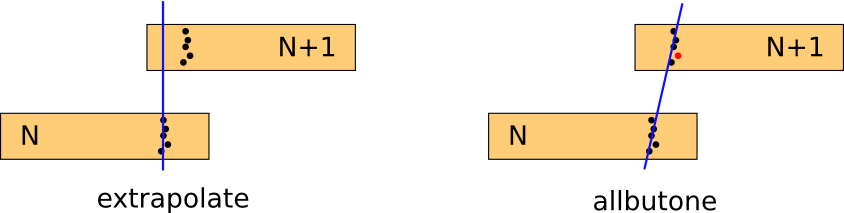
\includegraphics[width=0.7\linewidth]{fitting_methods.png}
\end{center}

Traditional fitting method (previous page): include hits on chamber $N$ in fit, align chamber $N+1$

\vspace{0.2 cm}
Tentative fitting method: include all hits in fit except the one whose
residual we calculate (residuals over uncertainty should be unit
Gaussian)

\vspace{0.2 cm}
\begin{columns}
\column{0.3\linewidth}
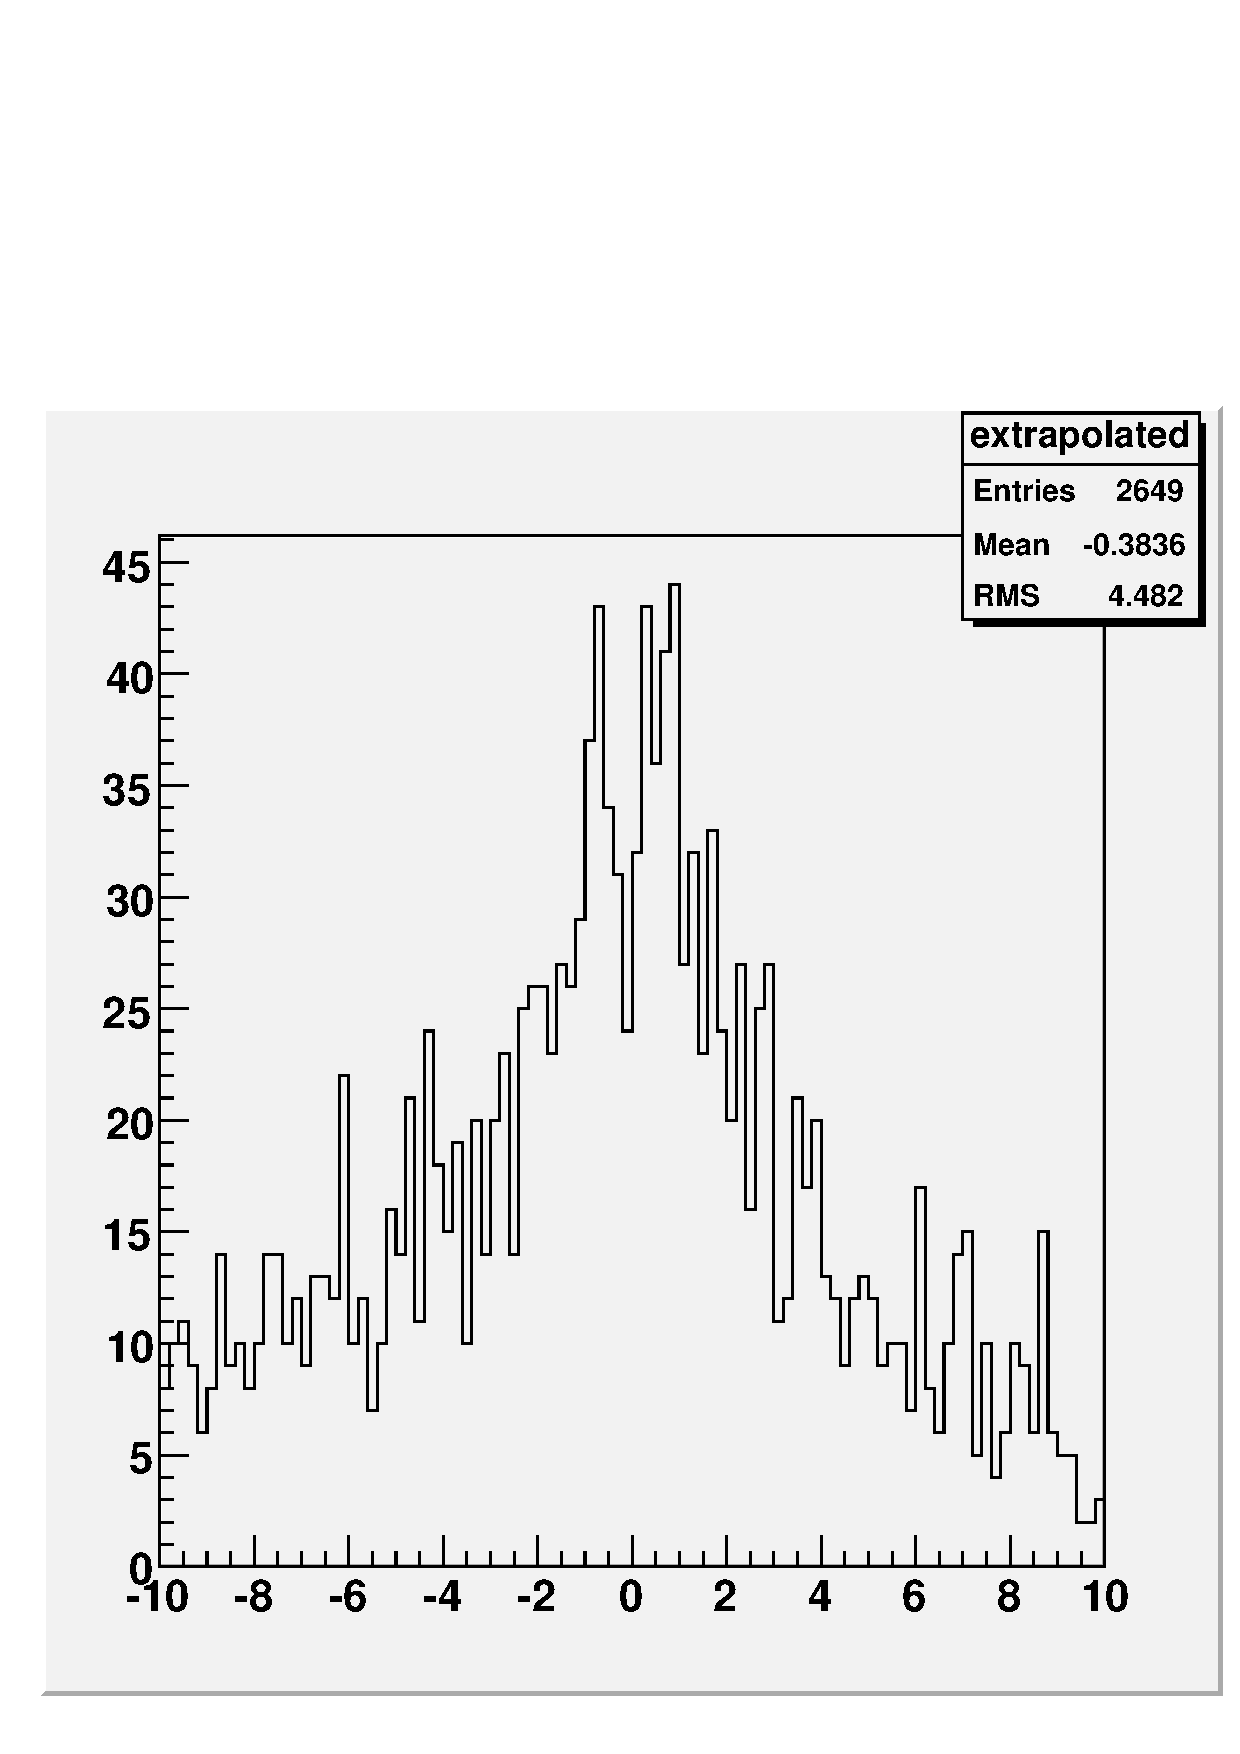
\includegraphics[width=\linewidth]{extrapolated_ME+211.pdf}

\column{0.3\linewidth}
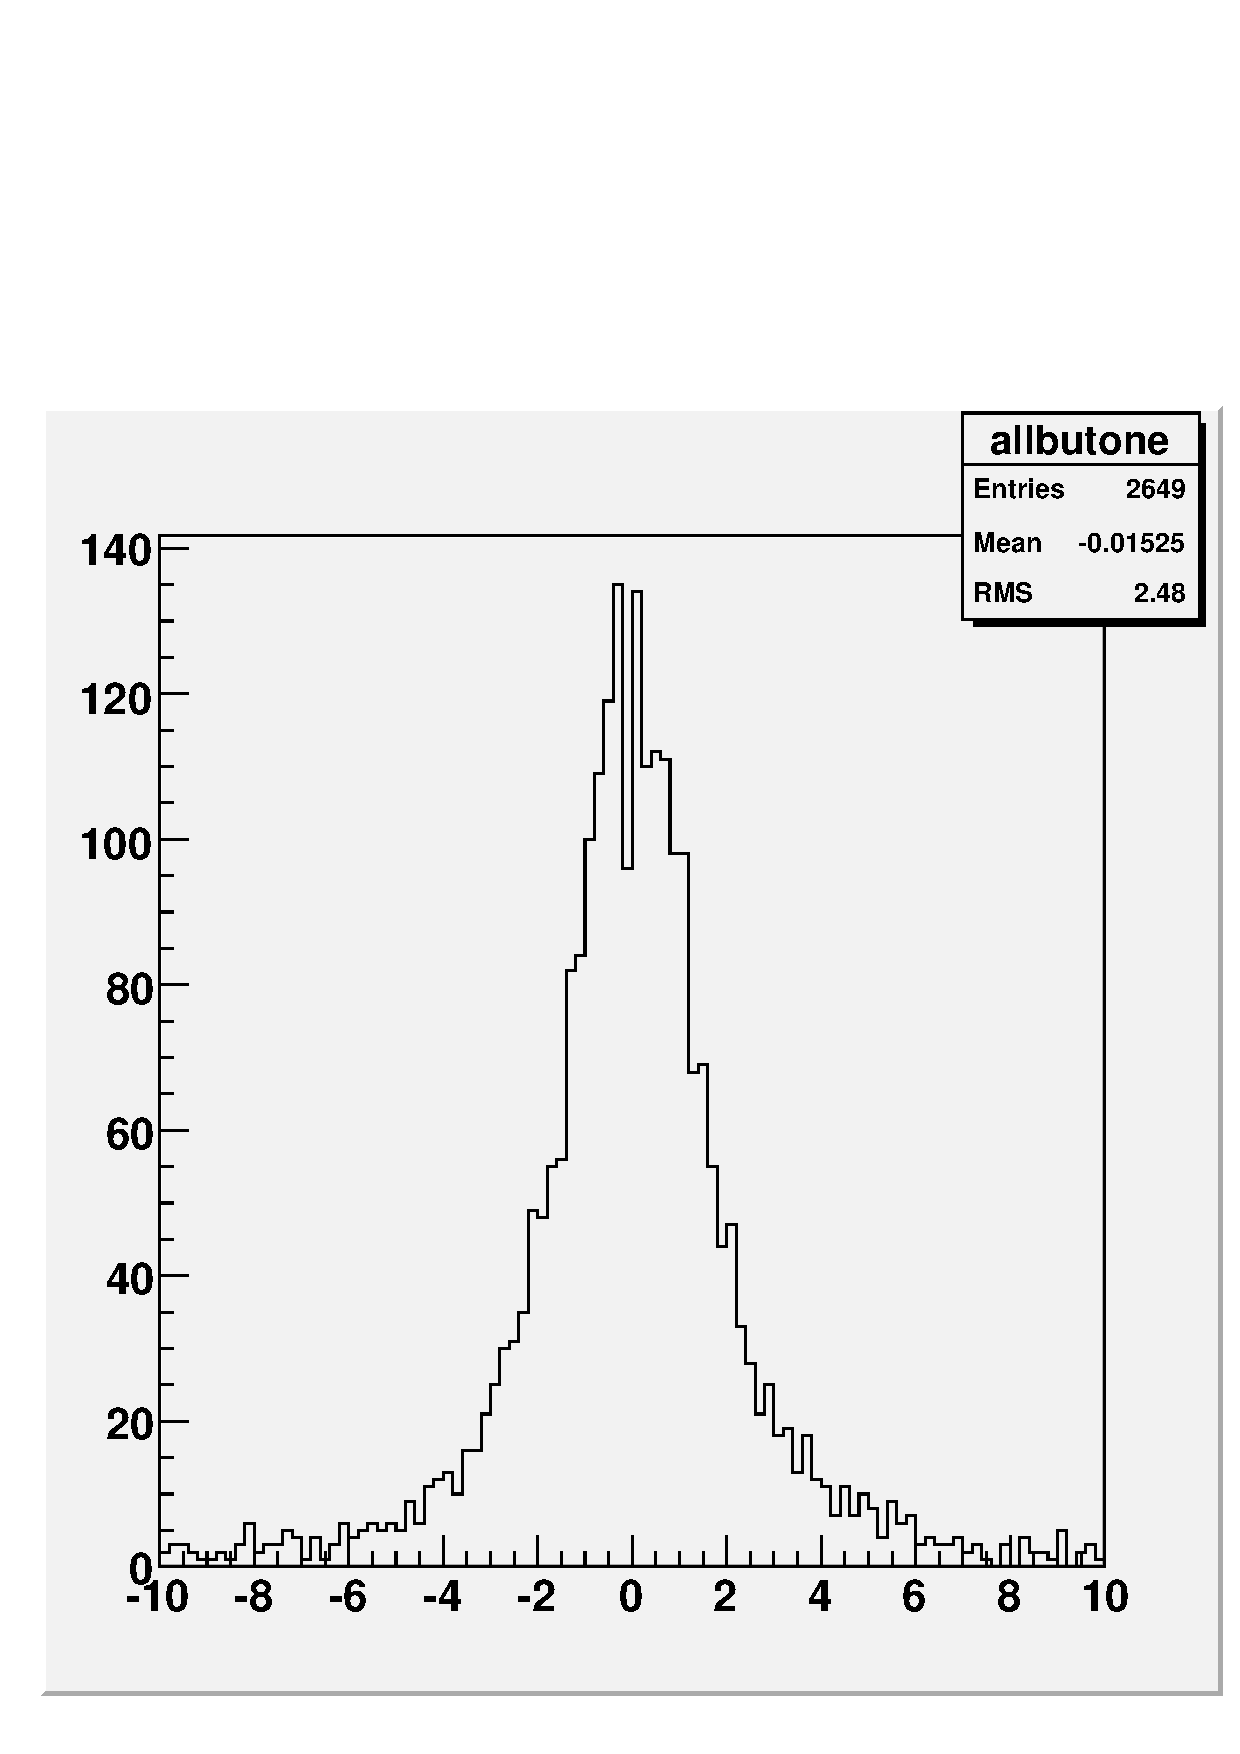
\includegraphics[width=\linewidth]{allbutone_ME+211.pdf}
\end{columns}

\scriptsize ME+2/1 chamber 1 residual over uncertainty in the two cases: 4.4 $\to$ 2.4
\end{frame}

\begin{frame}
\frametitle{Closure results with new fitter}
\small

\renewcommand{\arraystretch}{2}
\begin{tabular}{c c c c}
 & ME+2/1 wants to shrink & ME$-$2/1 shrink & ME$-$3/1 shrink \\\hline
Old fitter & 1600~$\mu$m & 6800~$\mu$m & 6000~$\mu$m \\
New fitter & 170~$\mu$m & 420~$\mu$m & 490~$\mu$m
\end{tabular}

\vfill
\begin{itemize}
\item Resolution improves by a factor of 2, but this bias decreases by
  a factor of 10--- it's not just because the track is more
  constrained
\item {\it However,} new fit does not yield misalignment, as old
  ``extrapolation fit'' did.  It will require iteration, and
  convergence is empirically slow.
\item Strike a balance by merely deweighting hits on the aligned
  chamber? (under study)
\end{itemize}
\end{frame}


%% chamber   before     after             (rphi in cm)
%%    1        0       0     (constraint)
%%    2        0      -0.0026
%%    3       -1.5    -0.0377
%%    4        0      -0.0024
%%    5       -1.     -0.0257
%%    6        0      -0.0071
%%    7        0      -0.0087
%%    8        0      -0.0055
%%    9        0      -0.0098
%%   10        1.      0.0179
%%   11        2.      0.0339
%%   12        0      -0.0156
%%   13        0      -0.0181
%%   14        0      -0.0298
%%   15        0      -0.0284
%%   16        0      -0.0182
%%   17        0      -0.0047
%%   18        0      -0.0056

\begin{frame}
\frametitle{What to do?}
\small
\begin{itemize}\setlength{\itemsep}{0.2 cm}
\item Find a deweighting factor that aligns chambers on a reasonable
  timescale without re-introducing the bias?  (hopefully)
\item Discover the origin of the bias, and if it's an internal
  misalignment, correct that too?  (too optimistic for a CMS Week
  timescale)
\item Evenly distribute error with matrix algorithm (fallback solution)
\item Use step-by-step algorithm with a fudge factor to do the same
  thing on incomplete rings?  (requires a strong assumption that true
  $r\phi$ misalignment doesn't have a coherent pattern, an assumption
  I don't want to make)
\item Complete rings in run 62232: ME+2/1, $-$2/1, and $-$3/1
\item Complete rings in whole beam$-$halo dataset: ME+2/1, +3/2, $-$2/1, $-$2/2, $-$3/1
\item CRUZET cosmic rays can add ME+2/2 and +3/2
\end{itemize}
\label{numpages}
\end{frame}

\end{document}
